\subsection{Coordinate polari}

\subsubsection{Coordinate polari sul piano}

\smallskip

\begin{tabular}{c p{0.5\textwidth}}
    \raisebox{-0.8\height}{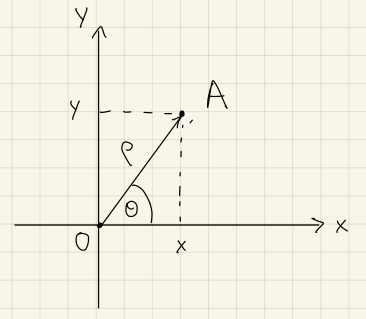
\includegraphics[width=0.40\textwidth]{coordinate-polari.png}}
     &
    \(A = (x,y) \in \R^2\) \hfill (coord.{ }cartesiane) \newline
    \(A = (\rho, \theta)\) \hfill (coord.{ }polari) \newline
    \hspace*{1cm}\(\downharpoonleft \ \downarrow \) \newline
    \hspace*{1cm}\(\downarrow \theta = \) angolo \newline
    \hspace*{1cm}\(\rho = \) lunghezza \newline
    \vspace{3mm} \newline
    \(\rho = \overline{OA} = d(A,\uzero) = \sqrt{x^{2}+y^{2}}\) \newline
    \(\theta = \arctan\left(\frac{y}{x}\right)\) \newline
\end{tabular}

\bigskip

Per passare da coordinare cartesiane a polari, basta usare la seguente relazione

\begin{equation*}
    \begin{cases}
        x - x_0 = \rho \cos\theta \\
        y - y_0 = \rho \sin\theta
    \end{cases}
    \ \implies
    \begin{cases}
        \rho = \sqrt{x^2 + y^2} \\
        \theta = \displaystyle \arctan\left(\frac{y}{x}\right) \pmod{2\pi}
    \end{cases} \\
\end{equation*}

\subsubsection{Limiti e coordinate polari}

\teorema{}{
    Sia \(f: D \subseteq \R^{2} \rightarrow \R \) e sia \(P_0=(x_0,y_0) \in D\) allora:

    \[
        \lim_{ (x,y) \to (x_0,y_0) } f(x,y) = l \ \iff \lim_{ \rho \to 0^{+} } f(x_0 + \rho\cos\theta ,\  y_0 + \rho\sin\theta ) = l
    \]

    \textbf{uniformemente rispetto a \(\theta \)}.
}

\defn{Uniformemente rispetto a \(\theta \)}{
    Dire che il limite è uniforme rispetto a \(\theta \) significa che il nostro limite (\(l\)) non dipende dalla scelta di \(\theta \), dove \(\theta \in (0,2\pi)\).
}

\defn{Limite finito con le coordinate polari}{
    Dire che

    \[
        \lim_{ \rho \to 0^{+} } f(x_0 + \rho\cos\theta ,\ y_0 + \rho\sin\theta ) = l
    \]

    significa quindi che:
    \medbreak{}

    \hspace*{5mm}
    \(\forall \varepsilon>0\),

    \hspace*{5mm}
    \(\exists \delta>0\) tale che \(\forall \rho \giventhat 0 < \rho < \delta\ ,  ~\forall \theta \in \lparen 0,2\pi \rbrack \)

    \hspace*{5mm}
    si ha: \(\big|f(x_0 + \rho\cos\theta ,\  y_0 + \rho\sin\theta  ) -l\big| < \varepsilon \)
}

Per dimostrare quanto abbiamo appena affermato, utilizzeremo il seguente procedimento che prende anche il nome di criterio del confronto.

\defn{Criterio del confronto}{
    Per far vedere che vale

    \[
        \lim_{ \rho \to 0^{+} } f(x_0 + \rho\cos\theta ,\ y_0 + \rho\sin\theta ) = l
    \]

    è sufficiente mostrare che esiste una funzione strettamente positiva \(g\) che dipende solo da \(\rho \), quindi \(\exists g(\rho) > 0\), tale che:

    \[
        0 \le \big|f(x_0 + \rho\cos\theta ,\  y_0 + \rho\sin\theta  ) -l\big| \le  g(\rho)
    \]

    dove si ha che:
    \[
        \lim_{\rho \to 0^+} g(\rho) \rightarrow 0
    \]

    Se accade che il limite dipende da \(\theta \), allora il limite non esiste.
}

\pagebreak

\subsubsection{Esempi ed esercizi}

\subsubsection*{Esempio precedente rifatto con le coordinate polari}

Avevamo già mostrato che il limite non esiste:

\[
    \lim_{ (x,y) \to (0,0) } \frac{xy}{x^{2}+y^{2}}
\]

\begin{equation*}
    \begin{cases}
        x = \rho\cos\theta \\
        y = \rho\sin\theta
    \end{cases}
\end{equation*}

il limite diventa:

\[
    \lim_{ \rho \to 0^{+} } \frac{\rho\cos\theta \cdot\rho\sin\theta }{\rho^{2}\cos^{2}\theta  + \rho^{2}\sin^{2}\theta } = \lim_{ \rho \to 0^{+} } \frac{\rho^{2}\cos\theta \sin\theta }{\rho^{2} \cdot (1)} = \frac{1}{2}\sin(2\theta)
\]

\(\implies \) limite dipende dalla scelta di \(\theta \).

\(\implies \) il limite non esiste dato che non è uniforme rispetto a \(\theta \)

\filbreak{}
\subsubsection*{Altro esempio}

Calcolare, se esiste, il seguente limite:

\[
    \lim_{ (x,y) \to (0,0) } \frac{xy}{\sqrt{x^{2}+y^{2}}}
\]

Trasformiamo in coordinate polari:

\[
    \lim_{ \rho \to 0^{+} } \frac{\rho\cos\theta \rho\sin\theta }{\sqrt{\rho^{2}}} = \lim_{ \rho \to 0^{+} } \frac{\rho^{2}\cos\theta \sin\theta }{\rho} = \lim_{ \rho \to 0^{+} } \rho\cos\theta\sin\theta = 0
\]

Dimostriamo che il candidato a essere limite, \(l=0\), esiste usando il criterio del confronto. Troviamo una \(g(\rho)\):

\[
    \rho\cos\theta\sin\theta = \rho\frac{\sin(2\theta)}{2} \le \left|\rho\frac{\sin(2\theta)}{2}\right| = \rho\left|\frac{\sin(2\theta)}{2}\right| \le \rho{\frac{1}{2}} = g(\rho)
\]

Questa \(g(\rho)\) dipende solo da \(\rho \) e \(\lim_{\rho \to 0^+} g(\rho) = 0\), quindi ok. Possiamo dunque dire che il limite esiste:

\[
    0 \le \left| \rho\cos\theta \sin\theta  -0 \right| \le \frac{1}{2}\rho
\]

\filbreak{}
\subsubsection*{Esercizio 1}

Calcolare, se esiste, il seguente limite:

\[
    \lim_{ (x,y) \to (0,0) } \frac{\arctan\left({(x+y)}^{2}\right)}{x^{2}}
\]

ricordo che \(\arctan(x) \sim x \text{ per } x\to0\);

consideriamo la funzione lungo l'asse x quindi con \(y=0\):

\[
    \lim_{ \begin{smallmatrix}(x,y) \to (0,0) \\ y=0\end{smallmatrix} } \frac{\arctan\left({(x+y)}^{2}\right)}{x^{2}}= \underbrace{\lim_{ x \to 0 } \frac{\arctan\left(x^{2}\right) }{x^{2}}}_{\text{limite notevole}} = 1
\]

vedo per la bisettrice (\(y=x\)):

\[
    \lim_{ \begin{smallmatrix}(x,y) \to (0,0) \\ y=x\end{smallmatrix} } \frac{\arctan\left({(x+y)}^{2}\right)}{x^{2}} = \lim_{ x \to 0 } \frac{\arctan\left({(x+x)}^{2}\right)}{x^{2}} = \lim_{ x \to 0 } \frac{\arctan\left({4x}^{2}\right)}{x^{2}} = 4
\]

quindi il limite non esiste.

\filbreak{}
\subsubsection*{Esercizio 2}

Calcolare, se esiste, il seguente limite:

\[
    \lim_{ (x,y) \to (0,0) } \frac{{(x+y)}^{2}}{x^{2}+y^{2}}
\]

vediamo cosa succede lungo l'asse x (\(y=0\)):

\[
    \lim_{ (x,y) \to (0,0) } \frac{{(x+y)}^{2}}{x^{2}+y^{2}} = \lim_{ x \to 0 } \frac{x^{2}}{x^{2}} = 1
\]

per \(y=x\):

\[
    \lim_{ (x,y) \to (0,0) } \frac{{(x+y)}^{2}}{x^{2}+y^{2}} = \lim_{ x \to 0 } \frac{{(x+x)}^{2}}{x^{2}+x^{2}} = 2
\]

quindi il limite non esiste.

\filbreak{}
\subsubsection*{Esercizio 3 {-} Definizione di continuità}

Calcolare, se esiste, il seguente limite:

\[
    \lim_{ (x,y) \to (0,0) } \frac{x^{2}-y^{2}}{x^{2}+y^{2}+5}
\]

Essendo questo un limite di funzioni continue (polinomi in due variabili), applicando la definizione di continuità posso dire che il limite è la funzione valutata nel punto di accumulazione.

Quindi il limite è \(= f(0,0) = 0\).

\filbreak{}
\subsubsection*{Esercizio 4 {-} Coordinate polari}

Calcolare, se esiste, il seguente limite:

\[
    \lim_{ (x,y) \to (0,0) } \frac{x\ln(1+x^{3})}{y(x^{2}+y^{2})}
\]

ricordo che \(\ln(1 + x) \sim x \text{ per } x\to0\);

passiamo in coordinate polari e dunque il limite diventa:

\begin{align*}
    \lim_{ \rho \to 0^{+} } \frac{\rho\cos\theta \cdot\ln\left(1+\rho^{3}\cos^{3}\theta \right)}{\rho\sin\theta \cdot\left(\rho^{2}\cos^{2}\theta  + \rho^{2}\sin^{2}\theta \right)} & = \lim_{ \rho \to 0^{+} } \frac{\rho\cos\theta \cdot\ln(1+\rho^{3}\cos^{3}\theta )}{\rho\sin\theta \cdot (\rho^{2}) }  \\
                                                                                                                                                                                     & = \lim_{ \rho \to 0^{+} } \frac{\rho\cos\theta \cdot \rho^{3}\cos^{3}\theta}{\rho^{3}\sin\theta }                      \\
                                                                                                                                                                                     & = \lim_{ \rho \to 0^{+} } \frac{\rho^{4}\cos^{4}\theta }{\rho^{3}\sin\theta } = \lim_{ \rho \to 0^{+} } \rho M(\theta)
\end{align*}

dove \(M(\theta) = \frac{\cos^{4}\theta }{\sin\theta }\) si nota che per ogni \(\theta \neq \pm \pi \) il limite è zero.

A questo punto non possiamo concludere subito che il limite non esiste, perché il denominatore non è sempre \(\ne 0\). Bisogna quindi analizzare, attraverso il teorema del confronto, il comportamento della funzione quando il denominatore è \(= 0\).

Ovvero, considerato il candidato a essere limite, 0, controlliamo se nei punti in cui la funzione non è definita il limite è uguale o meno.

\[
    \underset{\theta}{\sup} \bigl|\rho M(\theta)\bigr| = \sup\left|\rho \frac{\cos^{4}\theta }{\sin\theta }\right|
\]

se la nostra funzione, su \(\theta \in (0,2\pi)\) fosse finita, allora:

\[
    |M(\theta) | \le \bar{e}
\]

il \(\sup \) cioè è finito, e sono quindi a posto; ma \(M(\theta) \) non è limitata. Ad esempio, in \(\theta= \pi \) abbiamo un asintoto verticale:

\[
    \lim_{ \theta \to \pi } \frac{\cos^{4}\theta }{\sin\theta }= +\infty
\]

allora per studiare il limite vediamo che succede muovendoci verso l'origine lungo curve che sono tangenti all'asse x. Ovvero, curve (funzioni) la cui retta tangente in \((0,0)\) forma un angolo \(\theta = \pi \) con l'asse \(x\).

Consideriamo quindi \(y=x^{2}\):

\begin{align*}
    f(x,x^{2}) & = \frac{x\ln(1+x^{3})}{x^{2}(x^{2}+x^{4})} = \frac{\ln(1+x^{3})}{x^{3}(1+x^{2})} \overset{\text{per limite notevole}}{=} \frac{\cancel{x^3}}{\cancel{x^{3}}(1+x^{2})} \quad \xrightarrow[x \to 0]{}\  1 \implies \text{limite } \nexists
\end{align*}

\filbreak{}
\subsubsection*{Esercizio 5 {-} Limite con parametro reale}

Studiare l'esistenza del limite al variare del parametro reale \(\alpha \in \R \), con \(\alpha >0\):

\[
    \lim_{ (x,y) \to (1,0) } \frac{(x^2-2x+1)y}{{(x^2-2x+1+y^2)}^{\alpha}} =
    \lim_{ (x,y) \to (1,0) } \frac{{(x-1)}^2 y}{{\left({(x-1)}^2 + y^2\right)}^{\alpha}}
\]

Noto che questa funzione è definita su tutto \(\R \), e passo in coordinate polari:

\begin{equation*}
    \begin{cases}
        x = 1+\rho\cos\theta \\
        y = 0+\rho\sin\theta
    \end{cases}
\end{equation*}

allora:

\begin{align*}
    \lim_{ \rho \to 0^{+} } \frac{{(1 + \rho\cos\theta  -1 )}^{2} \rho\sin\theta }{{\left({(1+\rho\cos\theta  -1)}^{2}+\rho^{2}\sin^{2}\theta \right)}^{\alpha}} & = \lim_{ \rho \to 0^{+} } \frac{\rho^{2}\cos^{2}\theta \rho\sin\theta }{{\left(\rho^{2}\cos^{2}\theta +\rho^{2}\sin^{2}\theta \right)}^{\alpha}} \\
                                                                                                                                                                 & = \lim_{ \rho \to 0^{+} } \frac{\rho^{3}\cos^{2}\theta \sin\theta }{\rho^{2\alpha} \cdot 1}                                                      \\
                                                                                                                                                                 & = \lim_{ \rho \to 0^{+} } \rho^{3-2\alpha} \cos^{2}\theta \sin\theta
\end{align*}

Dato che \(\rho^x \xrightarrow[\rho \to 0^+]{} 0\) se \(x > 0\), analizziamo i vari casi ricordando che \(\alpha > 0\) per le condizioni iniziali:

\begin{itemize}
    \item Se \(3-2\alpha > 0\) ovvero \(\bm{0<\alpha < \frac{3}{2}}\):

          poiché \(\left\vert \cos^{2}\theta \sin\theta \right\vert \le 1\), attraverso il confronto diretto possiamo dire che:

          \[
              0 \le \left\vert\rho^{3-2\alpha}\cos^{2}\theta \sin\theta\right\vert = \rho^{3-2\alpha}\left\vert\cos^{2}\theta \sin\theta\right\vert \le \rho^{3-2\alpha} \to 0
          \]
          \(\implies \) il limite vale 0
    \item Se \(\bm{\alpha = \frac{3}{2}}\):

          \[
              \implies \lim_{\rho \to 0^+} \cancel{\rho^0} \cos^{2}\theta \sin\theta = \cos^{2}\theta \sin\theta
          \]

          dipende da \(\theta \) quindi il limite non esiste.
    \item Se \(\bm{\alpha > \frac{3}{2}}\):

          \[
              \alpha > \frac{3}{2} \implies \rho^{3-2\alpha} = \frac{1}{\rho^{2\alpha-3}}
          \]
          \[
              \implies \lim_{ \rho \to 0^{+} } \rho^{3-2\alpha} \cos^{2}\theta \sin\theta = \lim_{ \rho \to 0^{+} } \frac{\cos^{2}\theta \sin\theta}{\rho^{2\alpha-3}} = \pm \infty \ \text{ a seconda di } \theta
          \]

          Quindi il limite non esiste anche in questo caso. Da notare che se \(\sin\theta \) o \(\cos\theta \) fossero \(=0\), sarebbe più complesso, ma il limite comunque non esisterebbe.

\end{itemize}

\filbreak{}
\subsubsection*{Esercizio 6 {-} Studio di continuità}

Studiamo la continuità della seguente funzione nel suo dominio di definizione:

\[
    f(x,y)=
    \begin{cases}
        2x+3y+10 & \text{se}\ {(x-1)}^{2}+{(y-3)}^{2} \ge 4 \\
        x+4y+10  & \text{se}\ {(x-1)}^{2}+{(y-3)}^{2} < 4
    \end{cases}
\]

Abbiamo due piani, e una circonferenza. Devo vedere cosa succede a:
\[
    \lim_{ (x,y) \to (x_0,y_0) } x+4y+10 \qquad \forall (x_0,y_0) \in \{(x,y) \in \R^2 \giventhat {(x-1)}^{2}+{(y-3)}^{2} = 4\}
\]
Analizziamo l'intersezione tra questi due piani e la circonferenza:

\begin{equation*}
    \begin{cases}
        2x+3y+10 = x +4y +10 \\
        {(x-1)}^{2} + {(y-3)}^{2} = 4
    \end{cases}
\end{equation*}

verifichiamo se il sistema ha soluzione:
\begin{align*}
     & \begin{cases}
           x-y=0 \\
           {(x-1)}^{2} + {(y-3)}^{2} = 4
       \end{cases}\implies
    \begin{cases}
        x=y \\
        y^{2}-2y+1+y^{2}-6y+9=4
    \end{cases} \implies
    \begin{cases}
        x=y \\
        2y^{2}-8y + 6 = 0
    \end{cases}                 \\ \\
     & \implies \begin{cases}
                    x=y \\
                    y^{2}-4y+3=0
                \end{cases} \implies
    \begin{cases}
        x=y \\
        (y-3)(y-1) = 0
    \end{cases} \implies
    (x,y) \in \{(1,1), (3,3)\}
\end{align*}

Quindi possiamo concludere che la funzione \(f(x,y)\) è continua nei punti \((1,1)\) e \((3,3)\) ma non è continua su tutto \(\R^2\). Questo in quanto i due piani si intersecano solo in quei due punti, e non lungo tutta la circonferenza \({(x-1)}^{2}+{(y-3)}^{2} = 4\). Basta quindi prendere un qualsiasi altro punto sulla circonferenza, diverso da quei due, che il limite di \(x+4y+10\) in quel punto sarà diverso dalla funzione valutata nello stesso punto (dato che i piani non si intersecano).

\begin{center}
    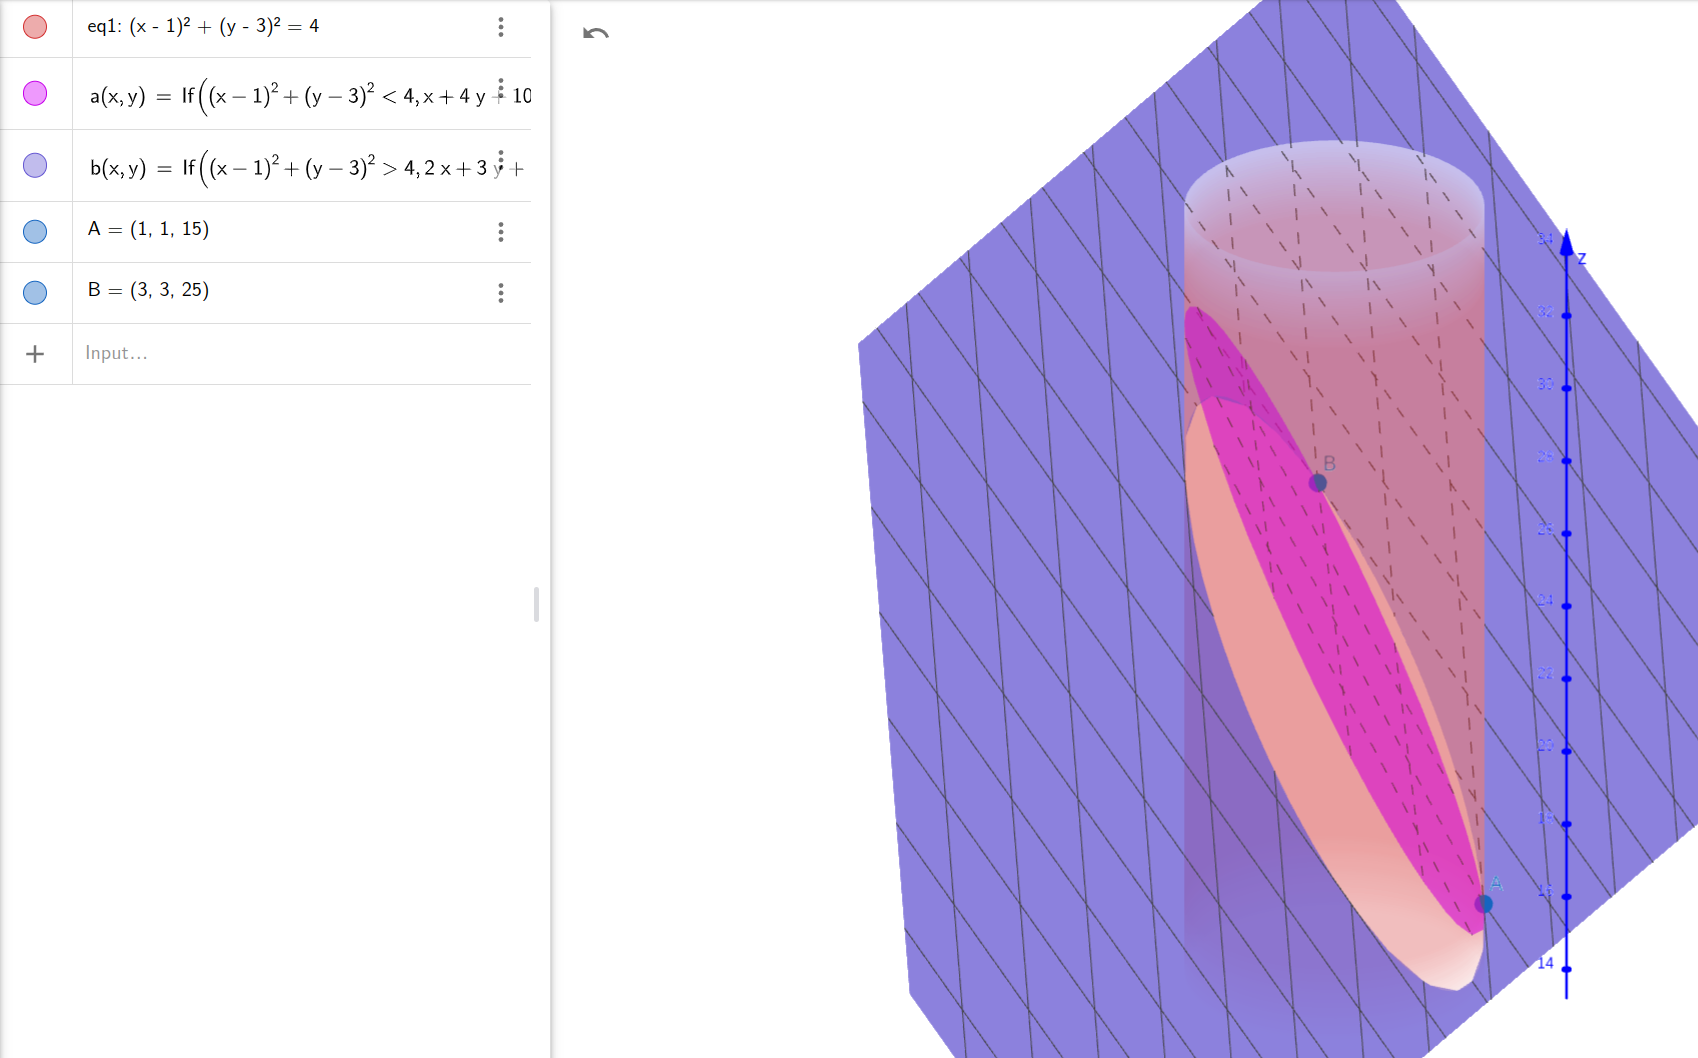
\includegraphics[width=0.85\textwidth]{limiti-esercizio-6.png}
\end{center}

\filbreak{}
\subsubsection*{Esercizio 7 {-} Studio di continuità}

Studiamo la continuità della seguente funzione, \(f: \R^2 \to \R \), nel suo dominio di definizione:

\[
    f(x,y) = \begin{cases*}
        0                                                                      & se \((x,y) = (1,1)\)   \\
        \displaystyle{\frac{e^{(x-1)+(y-1)} -1}{\sqrt{{(x-1)}^2 + {(y-1)}^2}}} & se \((x,y) \ne (1,1)\)
    \end{cases*}
\]

Affinché \(f(x,y)\) sia continua su tutto \(\R^2\) devo mostrare che

\[
    \lim_{(x,y) \to (1,1)} f(x,y) = \lim_{(x,y) \to (1,1)} \frac{e^{(x-1)+(y-1)} -1}{\sqrt{{(x-1)}^2 + {(y-1)}^2}} = f(1,1) = 0
\]

Guardiamo cosa fa la funzione lungo \(x=1\):

\[
    \lim_{\begin{smallmatrix}(x,y) \to (1,1) \\ x=1\end{smallmatrix}} f(x,y) =
    \lim_{y \to 1} \frac{e^{(y-1)} -1}{\sqrt{{(y-1)}^2}} =
    \lim_{y \to 1} \frac{e^{(y-1)} -1}{|y-1|} =
    \left[\frac{0}{0}\right] =
    \lim_{y \to 1} \frac{e^{(y-1)}}{\pm 1} = \pm 1
\]

Quindi il limite \(\nexists \)

Questo esercizio si poteva risolvere anche utilizzando le coordinate polari e facendo vedere che il limite non è uniforme rispetto a \(\theta \). Infatti, svolgendo i passaggi, il limite viene \(= \cos\theta + \sin\theta \)
